% Figure 2: architecture of the fault tolerant controller (the only manuscript figure that is not
% drawn from data). Every block is a module of the repository; rates are those of
% configs/controller_phase3.yaml and configs/robot_ipanema2_caspr.yaml.
% Build: pdflatex fig02_architecture.tex (scripts/paper_figures.py fig02 runs it).
\documentclass[tikz,border=3pt,10pt]{standalone}
\usepackage{amsmath}
\usepackage{mathptmx}
\usetikzlibrary{positioning,arrows.meta,calc}
\definecolor{ink}{HTML}{0B0B0B}
\definecolor{ink2}{HTML}{52514E}
\definecolor{edge}{HTML}{8A8984}
\definecolor{fillA}{HTML}{EEF4FC}
\definecolor{fillB}{HTML}{F5F4F0}
\definecolor{accent}{HTML}{256ABF}
\begin{document}
\footnotesize\hyphenpenalty=10000\exhyphenpenalty=10000
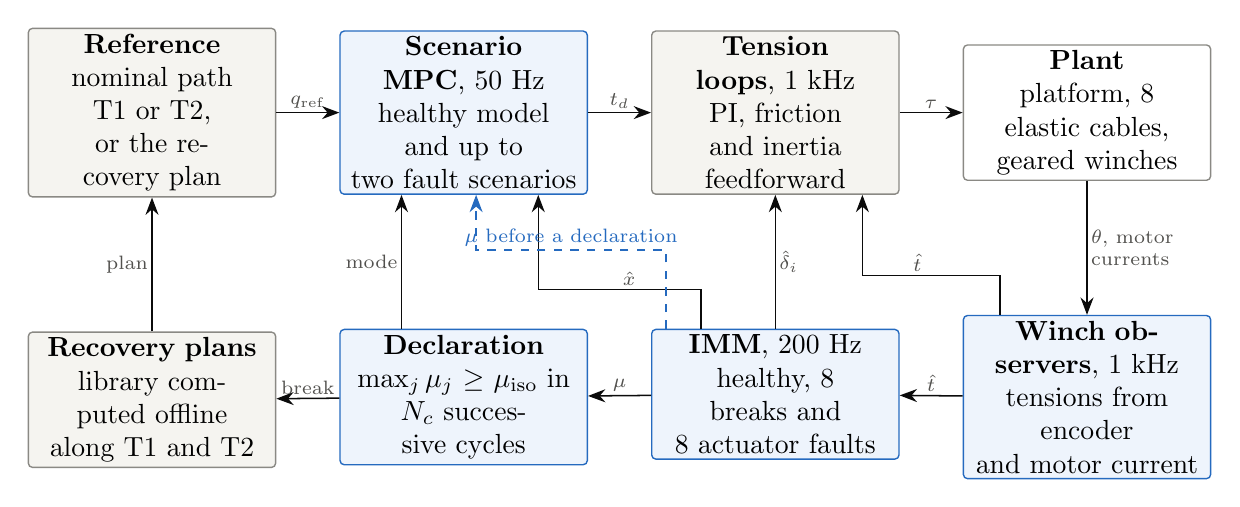
\begin{tikzpicture}[
  node distance=8mm,
  blk/.style={draw=edge, line width=0.5pt, rounded corners=1.5pt, fill=fillB, align=center,
              minimum height=12.5mm, text width=30mm, inner sep=2pt},
  est/.style={blk, fill=fillA, draw=accent},
  sig/.style={-{Stealth[length=2.2mm]}, line width=0.55pt, draw=ink},
  prob/.style={sig, draw=accent, dashed},
  lab/.style={font=\scriptsize, text=ink2, inner sep=1.2pt},
]
\node[blk] (ref) at (0,0) {\textbf{Reference}\\nominal path T1 or T2,\\or the recovery plan};
\node[est, right=of ref] (mpc) {\textbf{Scenario MPC}, 50 Hz\\healthy model and up to\\two fault scenarios};
\node[blk, right=of mpc] (loop) {\textbf{Tension loops}, 1 kHz\\PI, friction and inertia\\feedforward};
\node[blk, right=of loop, fill=white] (plant) {\textbf{Plant}\\platform, 8 elastic cables,\\geared winches};
\node[blk, below=17mm of ref] (plan) {\textbf{Recovery plans}\\library computed offline\\along T1 and T2};
\node[est, below=17mm of mpc] (dec) {\textbf{Declaration}\\$\max_j \mu_j \ge \mu_{\mathrm{iso}}$ in\\$N_c$ successive cycles};
\node[est, below=17mm of loop] (imm) {\textbf{IMM}, 200 Hz\\healthy, 8 breaks and\\8 actuator faults};
\node[est, below=17mm of plant] (eso) {\textbf{Winch observers}, 1 kHz\\tensions from encoder\\and motor current};
% forward path
\draw[sig] (ref) -- node[lab, above] {$q_{\mathrm{ref}}$} (mpc);
\draw[sig] (mpc) -- node[lab, above] {$t_d$} (loop);
\draw[sig] (loop) -- node[lab, above] {$\tau$} (plant);
% measurements and estimates
\draw[sig] (plant) -- node[lab, right, align=left] {$\theta$, motor\\currents} (eso);
\draw[sig] (eso) -- node[lab, above] {$\hat t$} (imm);
\draw[sig] ($(eso.north west)!0.15!(eso.north east)$) |- ++(0,5mm) -| node[lab, pos=0.3, above] {$\hat t$} ($(loop.south west)!0.85!(loop.south east)$);
% IMM outputs
\draw[sig] (imm) -- node[lab, above] {$\mu$} (dec);
\draw[sig] ($(imm.north west)!0.5!(imm.north east)$) -- node[lab, right, pos=0.5] {$\hat\delta_i$} ($(loop.south west)!0.5!(loop.south east)$);
\draw[sig] ($(imm.north west)!0.2!(imm.north east)$) -- ++(0,5mm) -| node[lab, pos=0.22, above] {$\hat x$} ($(mpc.south west)!0.8!(mpc.south east)$);
\draw[prob] ($(imm.north west)!0.06!(imm.north east)$) -- ++(0,10mm) -| node[lab, pos=0.25, above, text=accent] {$\mu$ before a declaration} ($(mpc.south west)!0.55!(mpc.south east)$);
% consequences of a declaration
\draw[sig] (dec) -- node[lab, above] {break} (plan);
\draw[sig] ($(dec.north west)!0.25!(dec.north east)$) -- node[lab, left] {mode} ($(mpc.south west)!0.25!(mpc.south east)$);
\draw[sig] (plan) -- node[lab, left] {plan} (ref);
\end{tikzpicture}
\end{document}
